\chapter{实践部分}
\section{TensorFlow例子}
\subsection{CNN手写体数据识别}
\subsection{mnist数据集}
手写体数据训练集有55000张手写体数据图片。测试集有10000张图片。每张图片是大小为32*32的灰度图片。
卷积神经网络结构:
\begin{itemize}
	\item 第一层卷积层:卷积核16个,卷积核大小为$5\times5$,strides=1,padding为SAME,激活函数为relu(输出大小为$28\times28\times16$)。
	\item 第一层池化层:池化层大小为2,strides为2($14\times14\times16$)。
第二层卷积层:卷积核32,大小为$5\times5$,strides=1,padding为SAME,激活函数为relu。($14\times14\times32$)
	\item 第二层池化层:池化层大小为2,strides为2($7\times7\times32$)。
	\item flatten:1568。
\end{itemize}
\begin{figure}[H]
	\includegraphics[scale=0.4]{./pic/chapter1/mnist_cnn.png}
\end{figure}
\begin{python}
import tensorflow as tf
import matplotlib.pyplot as plt
import numpy as np
from tensorflow.examples.tutorials.mnist import input_data

tf.set_random_seed(0)
np.random.seed(0)

BATCH_SIZE = 50
LR = 0.001
mnist = input_data.read_data_sets('/home/hpc/文档/mnist_tutorial/mnist',one_hot = True)
test_x = mnist.test.images[:2000]
test_y = mnist.test.labels[:2000]

tf_x = tf.placeholder(tf.float32,[None,28*28])
images = tf.reshape(tf_x,[-1,28,28,1])
tf_y = tf.placeholder(tf.int32,[None,10])
with tf.variable_scope('Conv1'):
    conv1 = tf.layers.conv2d(
            inputs = images,
            filters = 16,
            kernel_size = 5,
            strides = 1,
            padding = 'same',
            activation = tf.nn.relu
        )
    tf.summary.histogram('conv1',conv1)
with tf.variable_scope('pool1'):
    pool1 = tf.layers.max_pooling2d(
            conv1,
            pool_size=2,
            strides =2
        )
    tf.summary.histogram('max_pool1',pool1)
with tf.variable_scope('conv2'):
    conv2 = tf.layers.conv2d(pool1,32,5,1,'SAME',activation=tf.nn.relu)
    tf.summary.histogram('conv2',conv2)
with tf.variable_scope('pool2'):
    pool2 = tf.layers.max_pooling2d(conv2,2,2)
    tf.summary.histogram('max_pool',pool2)
with tf.variable_scope('flatten'):
    flat = tf.reshape(pool2,[-1,7*7*32])
with tf.variable_scope('output'):
    output = tf.layers.dense(flat,10)
with tf.variable_scope('loss_op'):
    loss = tf.losses.softmax_cross_entropy(onehot_labels=tf_y,logits=output)
    train_op = tf.train.AdamOptimizer(LR).minimize(loss)
    accuracy = tf.metrics.accuracy(labels = tf.argmax(tf_y,axis=1),predictions=tf.argmax(output,axis=1),)[1]
    tf.summary.scalar('loss',loss)
    tf.summary.scalar('accuracy',accuracy)
sess = tf.Session()
merge_op = tf.summary.merge_all()
init_op = tf.group(tf.global_variables_initializer(),tf.local_variables_initializer())
sess.run(init_op)
writer = tf.summary.FileWriter('./log',sess.graph)
for step in range(600):
    b_x,b_y = mnist.train.next_batch(BATCH_SIZE)
    _,loss_,result = sess.run([train_op,loss,merge_op],{tf_x:b_x,tf_y:b_y})
    writer.add_summary(result,step)
    if step%50 == 0:
        accuracy_,flat_representation = sess.run([accuracy,flat],{tf_x:test_x,tf_y:test_y})
        print('Step:',step,'| train loss:%.4f'%loss_,'|test accuracy:%.2f'%accuracy_)
test_output = sess.run(output,{tf_x:test_x[:10]})
pred_y = np.argmax(test_output,1)
\end{python}
LSTM 通常用来解决复杂的序列处理问题,比如包含了 NLP 概念(词嵌入、编码器等)的语言建模问题。这些问题本身需要大量理解,那么将问题简化并集中于在 TensorFlow 上实现 LSTM 的细节(比如输入格式化、LSTM 单元格以及网络结构设计),会是个不错的选择MNIST 就正好提供了这样的机会。其中的输入数据是一个像素值的集合。我们可以轻易地将其格式化,将注意力集中在 LSTM 实现细节上。

循环神经网络按时间轴展开的时候如下图:
\begin{figure}[H]
	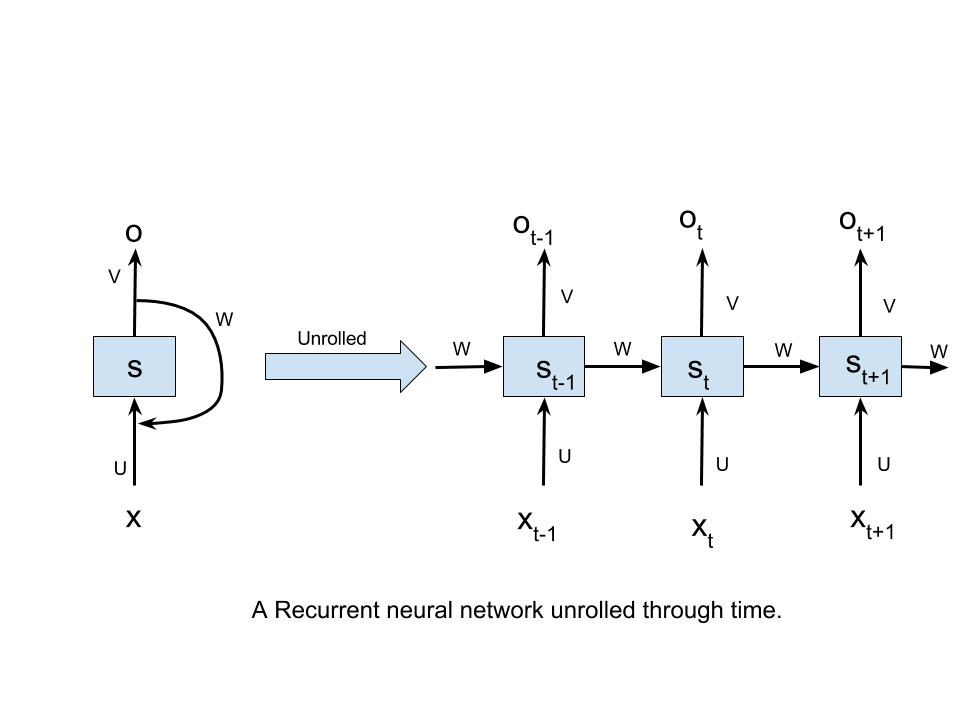
\includegraphics[scale=0.5]{Unrolled_RNN.png}
	\caption{循环神经网络的展开图}
\end{figure}
\begin{enumerate}
\item $x_t$ 代表时间步 t 的输入;
\item $s_t$ 代表时间步 t 的隐藏状态,可看作该网络的「记忆」;
\item $o_t$ 作为时间步 t 时刻的输出;
\item U、V、W 是所有时间步共享的参数,共享的重要性在于我们的模型在每一时间步以不同的输入执行相同的任务。
\end{enumerate}
当把 RNN 展开的时候,网络可被看作每一个时间步都受上一时间步输出影响(时间步之间存在连接)的前馈网络
在TensorFlow中基本的LSTM单元声明如下:
\lstinline[language=Python]{tf.contrib.rnn.BasicLSTMCell(null_units)}
这里,num\_units 指一个 LSTM 单元格中的单元数。num\_units 可以比作前馈神经网络中的隐藏层,前馈神经网络的隐藏层的节点数量等于每一个时间步中一个 LSTM 单元格内 LSTM 单元的 num\_units 数量。看下图:
\begin{figure}[H]
	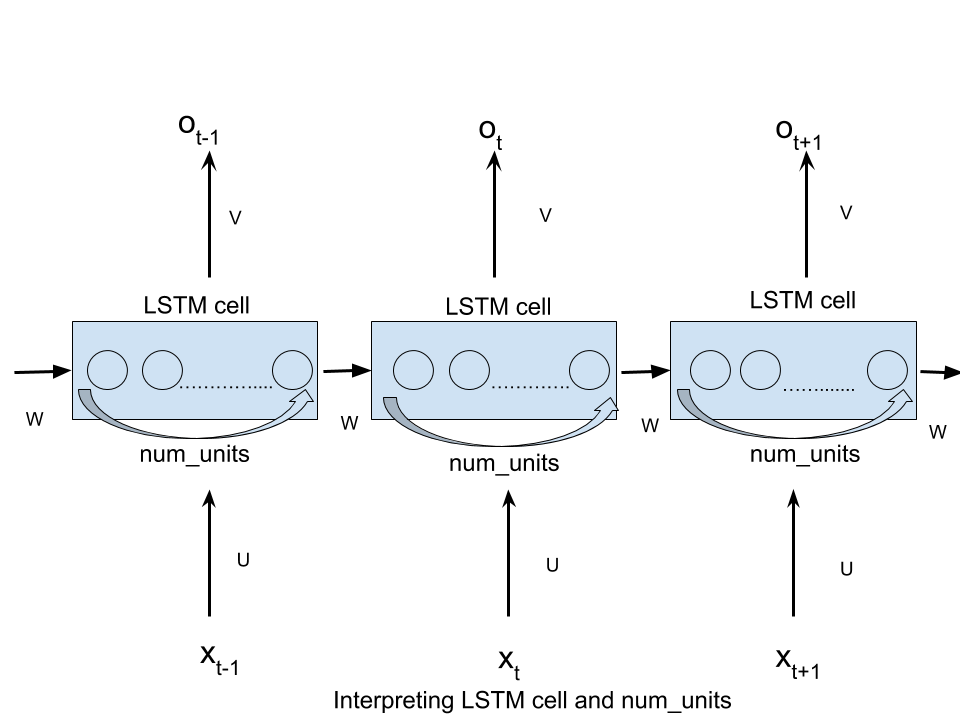
\includegraphics[scale=0.5]{num_units.png}
	\caption{LSTM单元和num\_units}
\end{figure}
每个num\_uints LSTM单元可以看做是一个标准的LSTM单元:
\begin{figure}[H]
	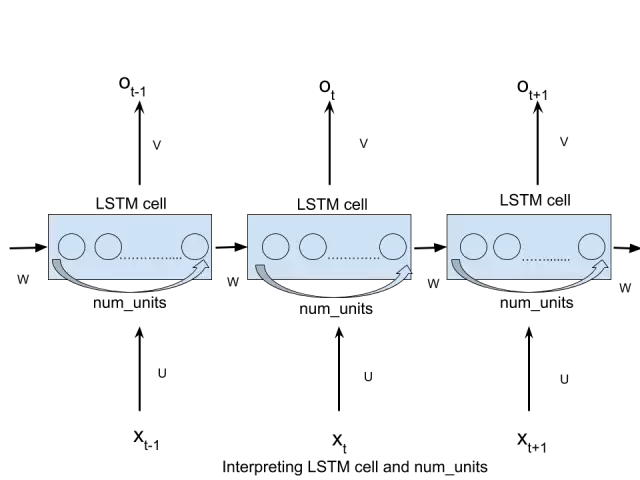
\includegraphics[scale=0.5]{lstm_unit.png}
	\caption{lstm单元}
\end{figure}
数据输入TensorFlow前先格式化,在TensorFlow中最简单的RNN形式是static\_rnn,在TensorFlow中定义如下:
\lstinline[language=Python]{tf.static_rnn(cell,inputs)}
inputs接受形状为[batch\_size,input\_size]的张量列表。列表的长度为将网络展开后的时间步数,即列表中每个元素都分别对应网络展开的时间步。比如MNIST数据集中,我们有$08\times28$像素的图像,每张图像都可以看成拥有258行28个像素的图像。我们将按28个时间步展开,以使在每个时间步中,可以输入一行28个像素(input\_size),二仅经过28个时间步输入整张图像。给定图像的batch\_size值,则每一个时间步将分别收到batch\_size个图像。如下图
\begin{figure}[H]
	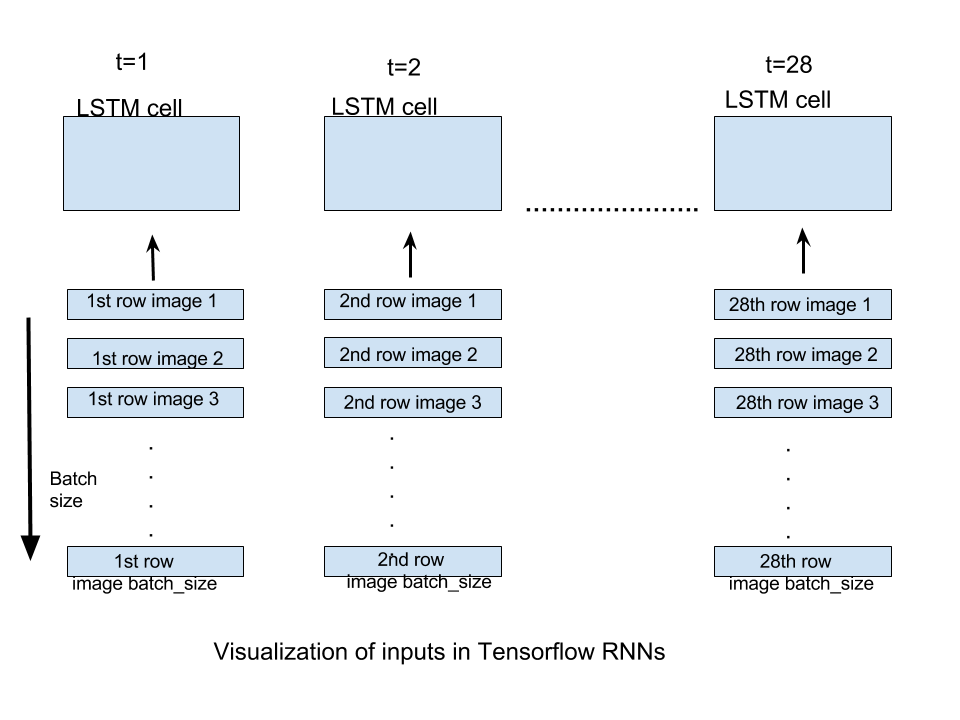
\includegraphics[scale=0.5]{inputs.png}
	\caption{可视化TensorFlow RNN}
\end{figure}
由 static\_rnn 生成的输出是一个形态为 [batch\_size,n\_hidden] 的张量列表。列表的长度为将网络展开后的时间步数,即每一个时间步输出一个张量。在这个实现中我们只需关心最后一个时间步的输出,因为一张图像的所有行都输入到 RNN,预测即将在最后一个时间步生成。
\subsection{卷积神经网络处理序列数据}
数据集\href{https://archive.ics.uci.edu/ml/machine-learning-databases/00240/UCI%20HAR%20Dataset.names}{(HAR Dataset)}介绍:该数据集来自于智能手机获取的人活动数据,追踪人的活动状态,总共有如下六种情况:
\begin{itemize}
\item 行走
\item 上楼梯
\item 下楼梯
\item 坐立
\item 站立
\item 平躺
\end{itemize}
数据有来自加速度计和陀螺仪的数据,数据集分为测试集和训练集,训练集数据有7352个数据,数据包括如下:
\begin{itemize}
	\item body\_acc:从总的加速度中减去重力获得的加速度信号(128个值组成)
	\item body\_gyro:陀螺仪获得角速度(128个值组成)
	\item total\_acc:总的加速度(128个值组成)
\end{itemize}每个数据有128个特征。测试集有2947个数据

卷积神经网络架构如下:
\begin{figure}[H]
\includegraphics[scale=0.5]{HAR_cnn.png}
\caption{CNN处理HAR数据的架构}
\end{figure}
数据预处理模块:
\lstinputlisting[language=Python]{./code/har/utilities.py}
神经网络实现模块:
\lstinputlisting[language=Python]{./code/har/cnn_har.py}
\subsection{LSTM处理序列数据}
LSTM架构如下:
\begin{figure}[H]
	\includegraphics[scale=0.5]{HAR_lstm.png}
	\caption{lstm架构图}
\end{figure}
\lstinputlisting[language=Python]{./code/har/lstm_har.py}
CNN和LSTM结合
\lstinputlisting[language=Python]{./code/har/cnn_lstm_har.py}


